\documentclass[11pt,a4paper]{article}
\usepackage[utf8]{inputenc}
\usepackage[margin=1in]{geometry}
\usepackage{graphicx}
\usepackage{hyperref}
\usepackage{listings}
\usepackage{xcolor}
\usepackage{tcolorbox}
\usepackage{enumitem}
\usepackage{amsmath}
\usepackage{booktabs}
\usepackage{fancyhdr}
\usepackage{titlesec}

% Code listing style
\lstset{
    basicstyle=\ttfamily\small,
    breaklines=true,
    frame=single,
    backgroundcolor=\color{gray!10},
    keywordstyle=\color{blue},
    commentstyle=\color{green!60!black},
    stringstyle=\color{red},
    numbers=left,
    numberstyle=\tiny\color{gray},
    tabsize=2
}

% Define JavaScript language for listings
\lstdefinelanguage{JavaScript}{
  keywords={typeof, new, true, false, catch, function, return, null, catch, switch, var, if, in, while, do, else, case, break, const, let, await, async, export, import, class, extends, super, this},
  keywordstyle=\color{blue}\bfseries,
  ndkeywords={boolean, throw, import, export, implements, interface, module, require},
  ndkeywordstyle=\color{blue}\bfseries,
  identifierstyle=\color{black},
  sensitive=false,
  comment=[l]{//},
  morecomment=[s]{/*}{*/},
  commentstyle=\color{green!60!black}\ttfamily,
  stringstyle=\color{red}\ttfamily,
  morestring=[b]',
  morestring=[b]"
}

% Define json language for listings
\lstdefinelanguage{json}{
    basicstyle=\ttfamily\small,
    captionpos=b,
    showstringspaces=false,
    breaklines=true,
    frame=single,
    literate=
     *{0}{{{\color{blue}0}}}{1}
      {1}{{{\color{blue}1}}}{1}
      {2}{{{\color{blue}2}}}{1}
      {3}{{{\color{blue}3}}}{1}
      {4}{{{\color{blue}4}}}{1}
      {5}{{{\color{blue}5}}}{1}
      {6}{{{\color{blue}6}}}{1}
      {7}{{{\color{blue}7}}}{1}
      {8}{{{\color{blue}8}}}{1}
      {9}{{{\color{blue}9}}}{1}
      {:}{{{\color{black}{:}}}}{1}
      {,}{{{\color{black}{,}}}}{1}
      {\{}{{{\color{black}{\{}}}}{1}
      {\}}{{{\color{black}{\}}}}}{1}
      {[}{{{\color{black}{[}}}}{1}
      {]}{{{\color{black}{]}}}}{1},
}

% Define yaml language for listings
\lstdefinelanguage{yaml}{
  keywords={true,false,null,y,n},
  keywordstyle=\color{blue}\bfseries,
  basicstyle=\ttfamily\small,
  sensitive=false,
  comment=[l]{\#},
  morecomment=[s]{/*}{*/},
  commentstyle=\color{green!60!black}\ttfamily,
  stringstyle=\color{red}\ttfamily,
  moredelim=[l][\color{orange}]{\&},
  moredelim=[l][\color{magenta}]{*},
  moredelim=**[il][\color{blue}]{:},
  morestring=[b]',
  morestring=[b]",
  literate={\ -\ }{{\ -\ }}3
}

% Header and footer
\pagestyle{fancy}
\fancyhf{}
\rhead{NexGuard: Human-Governed AI Code Orchestration}
\lhead{\thepage}
\renewcommand{\headrulewidth}{0.4pt}

% Title formatting
\titleformat{\section}
  {\Large\bfseries}{\thesection}{1em}{}
\titleformat{\subsection}
  {\large\bfseries}{\thesubsection}{1em}{}

% Hyperlink colors
\hypersetup{
    colorlinks=true,
    linkcolor=blue,
    urlcolor=blue,
    citecolor=blue
}

\title{
    \Huge\textbf{NexGuard} \\ 
    \vspace{0.5cm}
    \Large Human-Governed AI Coding Agent Orchestration Platform \\
    \vspace{0.5cm}
    \large Project Documentation - DLWeek
}
\author{Team PPPPP}
\date{}

\begin{document}

\maketitle
\thispagestyle{empty}

\vspace{0.5cm}
\begin{center}
\Large\textbf{Summary}
\end{center}
\vspace{0.3cm}

\noindent NexGuard is a production-ready platform that intercepts AI-generated code changes, scores their blast radius using machine learning, and routes them through a risk-tiered human approval system. Unlike traditional CI/CD pipelines that act \textit{after} deployment, NexGuard operates \textit{before} code reaches version control, providing human oversight of AI agents during the development phase. This document details our methodology, implementation, and testing procedures from building a full-stack system that covers the entire Software Development Lifecycle (SDLC): development, testing, deployment, incident response, and governance.

\vspace{0.5cm}

\newpage
\tableofcontents
\newpage

% ============================================================================
\section{Executive Summary}
% ============================================================================

\subsection{Problem Statement}
As AI coding agents like GitHub Copilot, Cursor, and OpenAI Codex become more capable, they are transitioning from auto-complete tools to autonomous code generators. However, these agents lack awareness of production systems, security implications, and business context. Blindly executing AI-generated code poses significant risks:

\begin{itemize}[leftmargin=*]
    \item \textbf{Security vulnerabilities} --- AI may introduce authentication bypasses or SQL injection
    \item \textbf{System instability} --- Breaking changes to critical infrastructure
    \item \textbf{Data loss} --- Destructive database migrations or data deletion
    \item \textbf{Compliance violations} --- Changes that bypass audit trails or regulatory requirements
\end{itemize}

\subsection{Our Solution}
NexGuard introduces a \textbf{risk-tiered approval system} that intercepts every AI-generated code proposal and routes it through one of three paths:

\begin{tcolorbox}[colback=green!10,colframe=green!60!black,title=GREEN Tier (Auto-Execute)]
Low-risk changes (documentation, comments, tests) execute automatically with logging only.
\end{tcolorbox}

\begin{tcolorbox}[colback=yellow!10,colframe=yellow!60!black,title=YELLOW Tier (Notify + Veto)]
Medium-risk changes (config updates, performance optimizations) execute with notification and 1-hour veto window.
\end{tcolorbox}

\begin{tcolorbox}[colback=red!10,colframe=red!60!black,title=RED Tier (Hard Block)]
High-risk changes (authentication, database migrations, production config) require explicit human approval before execution.
\end{tcolorbox}

\subsection{Key Innovation}
We combine \textbf{three ML models} (CodeBERT classifier, autoencoder anomaly detector, cosine similarity) with \textbf{three GPT-4o agents} (code generation, review, documentation) and \textbf{Jira Cloud integration} to create a defense-in-depth system where:
\begin{enumerate}
    \item \textbf{Issues flow from Jira} → NexGuard webhook → risk scoring pipeline
    \item \textbf{AI generates} proposals with full context from RAG (Retrieval-Augmented Generation)
    \item \textbf{ML scores} blast radius using fine-tuned CodeBERT and anomaly detection
    \item \textbf{Humans approve} anything risky through Slack interactive cards
    \item \textbf{System logs} everything in an append-only audit trail for compliance
\end{enumerate}

\subsection{What We Built}
A complete full-stack platform consisting of:
\begin{itemize}
    \item \textbf{Node.js Backend} (TypeScript + Express) with 15 REST endpoints, 5 AI agents, 3 services
    \item \textbf{Jira Cloud Integration} via webhooks with ADF text extraction and smart repo mapping
    \item \textbf{Python ML Sidecar} (FastAPI) with 3 trained models (classifier, autoencoder, similarity)
    \item \textbf{Next.js Dashboard} with real-time audit feed and approval interface
    \item \textbf{Slack Integration} with Block Kit approval cards and interactive components
    \item \textbf{PostgreSQL + Redis + ChromaDB} for data persistence and vector search
    \item \textbf{GitHub Integration} via Octokit for branch creation and PR management
    \item \textbf{Policy-Driven Governance} with YAML config for risk thresholds and fail-safe patterns
    \item \textbf{Compliance Reporting} with aggregate statistics and audit trail exports
    \item \textbf{Incident Management} with 45s hotfix generation and emergency PR workflow
\end{itemize}

% ============================================================================
\newpage
\section{System Architecture}
% ============================================================================

\subsection{High-Level Design}
NexGuard follows a microservices architecture with clear separation of concerns:
\begin{figure}[h!]
    \centering
    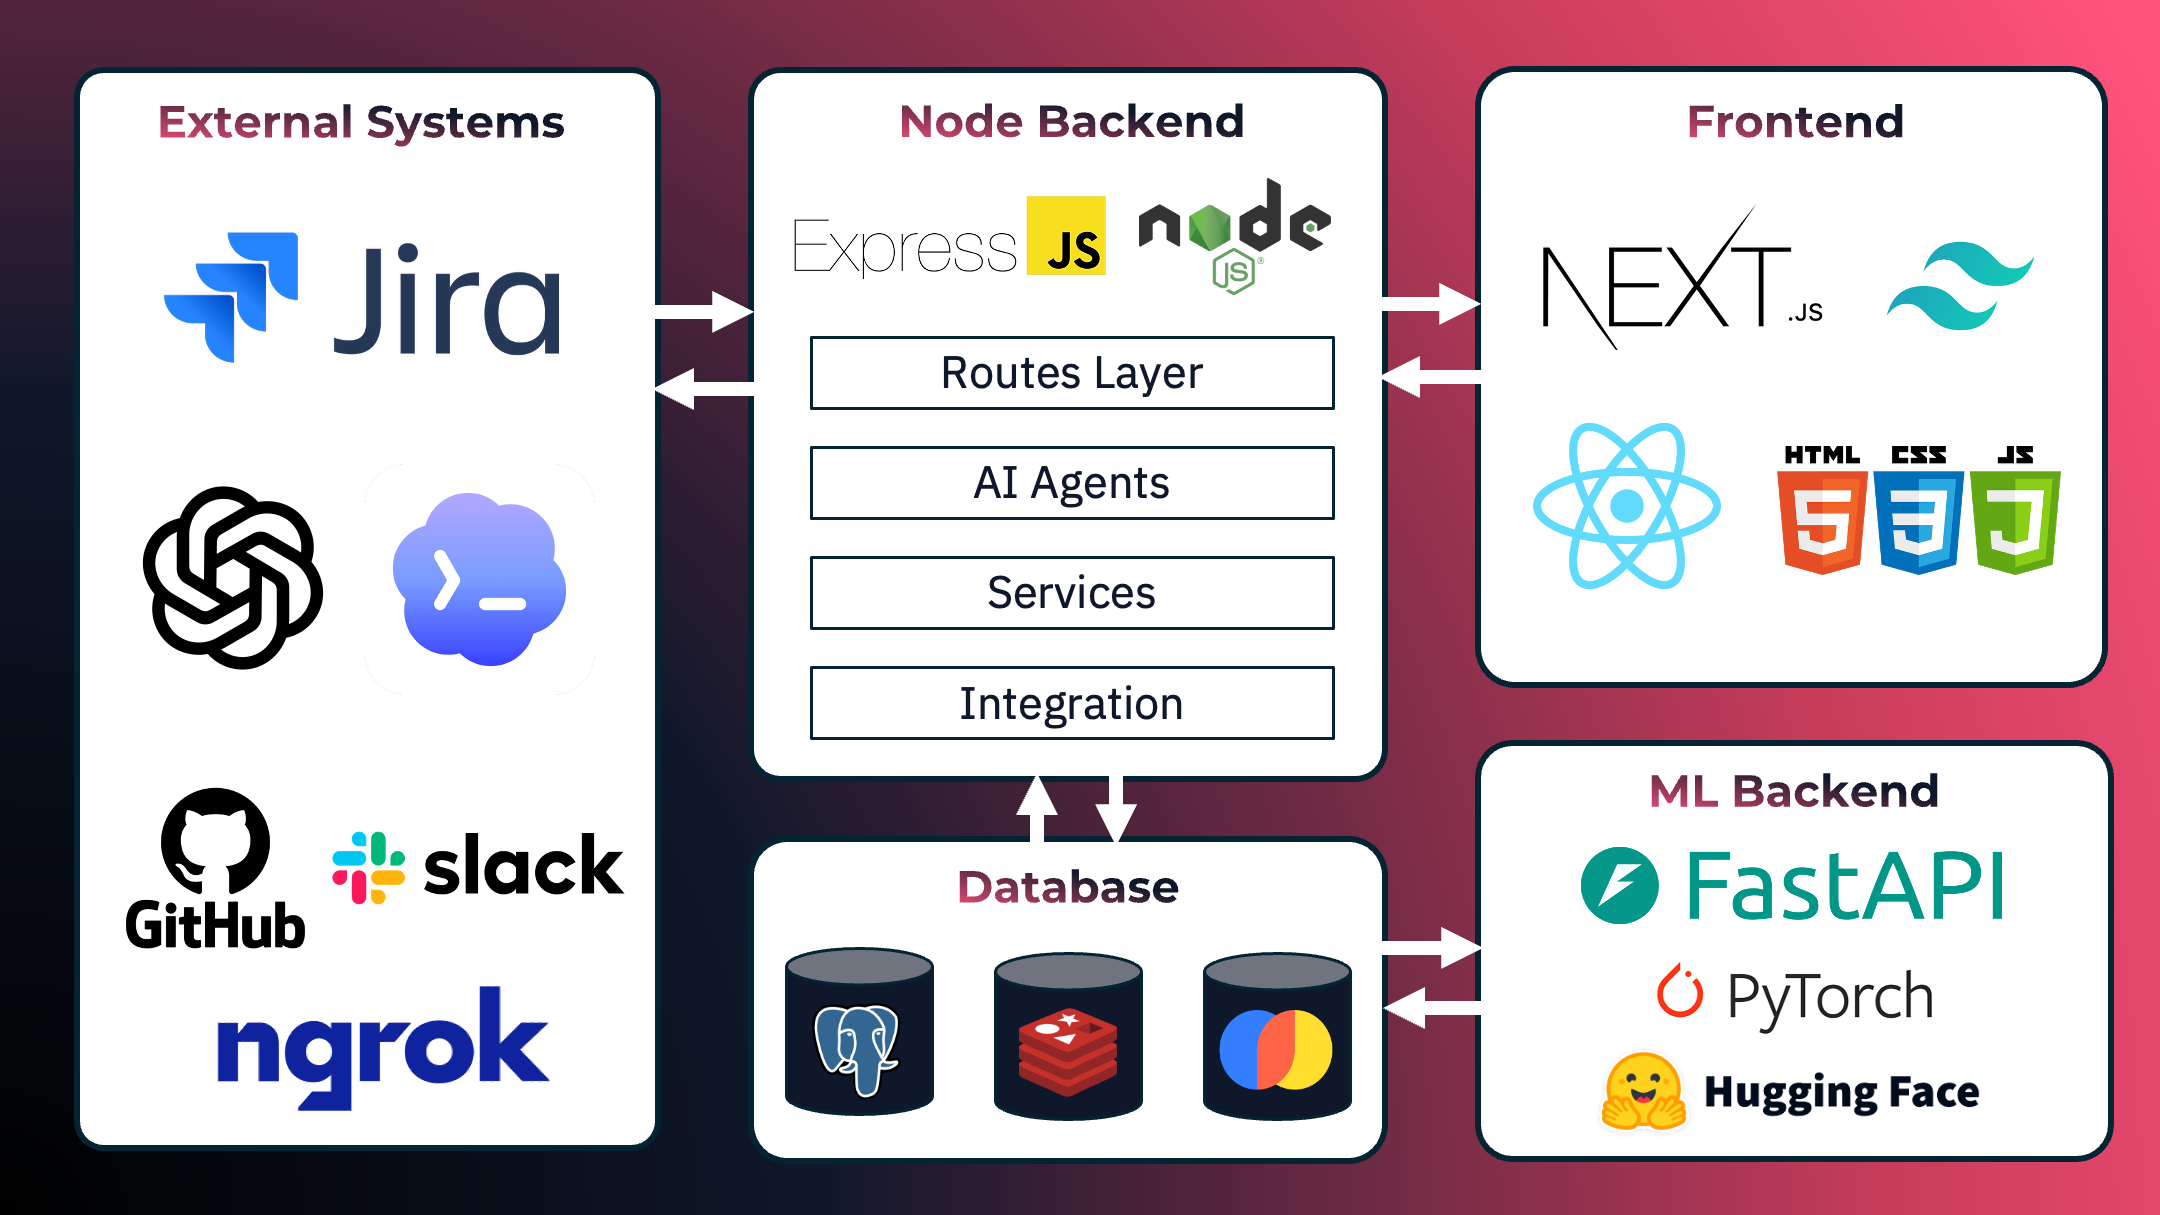
\includegraphics[width=1\linewidth]{Architecture.png}
    \caption{NexGuard System Architecture}
    \label{fig:placeholder}
\end{figure}
% \begin{figure}[h!]
% \centering
% \begin{verbatim}
% +------------------------------------------------------------------+
% |                      NexGuard Platform                           |
% |                                                                  |
% |  +----------+     +---------------+     +-----------------+     |
% |  |  Ticket  |---->|  Node.js      |<--->|  Python ML      |     |
% |  |  Input   |     |  Backend      |     |  Sidecar        |     |
% |  | (Jira)   |     |  Port 3000    |     |  Port 8001      |     |
% |  +----------+     +-------+-------+     +-----------------+     |
% |                           |                                      |
% |          +----------------+------------------+                   |
% |          |                |                  |                   |
% |     +----+----+      +----+----+      +------+------+           |
% |     |PostgreSQL|     | Redis  |      |ChromaDB      |           |
% |     |  5433   |      |  6379  |      |(Vector)      |           |
% |     +---------+      +--------+      +-------------+            |
% |                                                                  |
% |     External: OpenAI GPT-4o | GitHub (Octokit) | Slack         |
% +------------------------------------------------------------------+
% \end{verbatim}
% \caption{NexGuard System Architecture}
% \end{figure}

\subsection{Technology Stack}

\subsubsection{Backend (Node.js)}
\begin{itemize}
    \item \textbf{Runtime:} Node.js 20+ with TypeScript 5.0
    \item \textbf{Web Framework:} Express.js 4.18
    \item \textbf{ORM:} Prisma 5.0 (type-safe database client)
    \item \textbf{Cache:} Redis 7 (session storage, planned: job queue with BullMQ)
    \item \textbf{Vector DB:} ChromaDB 1.5 (RAG embeddings)
    \item \textbf{Config:} YAML-based policy file (risk thresholds, fail-safe patterns)
\end{itemize}

\subsubsection{ML Sidecar (Python)}
\begin{itemize}
    \item \textbf{Runtime:} Python 3.11 with FastAPI
    \item \textbf{ML Framework:} PyTorch 2.0 (autoencoder)
    \item \textbf{Transformers:} HuggingFace 4.30 (CodeBERT)
    \item \textbf{Embeddings:} OpenAI text-embedding-3-small
    \item \textbf{Similarity:} scikit-learn 1.3 (cosine distance)
\end{itemize}

\subsubsection{Frontend \& Integrations}
\begin{itemize}
    \item \textbf{Dashboard:} Next.js 14 with React 18
    \item \textbf{Database:} PostgreSQL 15 (primary data store)
    \item \textbf{Issue Tracker:} Jira Cloud (webhook integration, ADF parsing)
    \item \textbf{Notifications:} Slack Webhooks + Interactive Components
    \item \textbf{Version Control:} GitHub via Octokit REST API
    \item \textbf{AI:} OpenAI API (GPT-4o for agents)
\end{itemize}

\subsection{Component Breakdown}

\subsubsection{Routes Layer (API Endpoints)}
\begin{table}[h!]
\centering
\begin{tabular}{@{}lll@{}}
\toprule
\textbf{Endpoint} & \textbf{Method} & \textbf{Purpose} \\
\midrule
\texttt{/intake} & POST & Submit development ticket (direct) \\
\texttt{/intake/jira} & POST & Accept Jira webhook payloads \\
\texttt{/incident} & POST & Declare production incident \\
\texttt{/incident} & GET & List all incidents with hotfixes \\
\texttt{/incident/:id} & GET & Get single incident details \\
\texttt{/incident/:id/apply/:hotfixId} & POST & Apply a hotfix (creates PR) \\
\texttt{/incident/:id/resolve} & POST & Manually resolve an incident \\
\texttt{/approve/:id} & GET & Approve proposal (Slack callback) \\
\texttt{/reject/:id} & GET & Reject proposal (Slack callback) \\
\texttt{/veto/:id} & GET & Veto YELLOW-tier auto-execution \\
\texttt{/diff/:id} & GET & View proposal diff + metadata \\
\texttt{/audit/feed} & GET & Real-time audit log stream \\
\texttt{/audit/report} & GET & Generate compliance report \\
\texttt{/slack/events} & POST & Interactive component callbacks \\
\texttt{/health} & GET & System health check \\
\bottomrule
\end{tabular}
\caption{API Endpoints}
\end{table}

\subsubsection{AI Agents}
\begin{enumerate}
    \item \textbf{Codex Agent} (\texttt{agents/codex.ts})
    \begin{itemize}
        \item Generates code diffs from natural language tickets
        \item Uses GPT-4o with RAG context from ChromaDB
        \item Outputs diff, summary, risk list, confidence score
    \end{itemize}
    
    \item \textbf{RAG Agent} (\texttt{agents/rag.ts})
    \begin{itemize}
        \item Embeds tickets using OpenAI text-embedding-3-small
        \item Queries ChromaDB for similar past proposals
        \item Provides context to Codex for better generation
    \end{itemize}

    \newpage
    \item \textbf{Reviewer Agent} (\texttt{agents/reviewer.ts})
    \begin{itemize}
        \item Second independent GPT-4o pass on proposal
        \item Adjusts risk score based on overlooked factors
        \item Merges with ML classifier for final tier
    \end{itemize}
    
    \item \textbf{Incident Agent} (\texttt{agents/incident.ts})
    \begin{itemize}
        \item Analyzes production logs during incidents
        \item Generates 3-5 ranked hotfix candidates
        \item 45-second countdown for human selection
    \end{itemize}
    
    \item \textbf{Communication Agent} (\texttt{agents/communication.ts})
    \begin{itemize}
        \item Always reads from AuditLog (append-only truth)
        \item \textbf{generatePRDescription()} --- Creates PR descriptions with:
        \begin{itemize}
            \item Summary of changes and rationale
            \item Risk assessment with reviewer notes
            \item Audit trail of approval flow
            \item Testing recommendations
        \end{itemize}
        \item \textbf{generatePostmortem()} --- Creates incident postmortems with:
        \begin{itemize}
            \item Timeline of events from audit logs
            \item Root cause analysis
            \item Hotfixes evaluated and applied
            \item Action items for prevention
            \item Lessons learned (blame-free)
        \end{itemize}
        \item \textbf{generateChangelog()} --- Produces release changelogs:
        \begin{itemize}
            \item Groups proposals by category (Features, Fixes, Breaking Changes)
            \item User-friendly language
            \item Date ranges and risk tiers
            \item Only includes EXECUTED proposals
        \end{itemize}
    \end{itemize}
\end{enumerate}

\subsubsection{ML Models (Python Sidecar)}
\begin{enumerate}
    \item \textbf{Blast Radius Classifier} (\texttt{classify.py})
    \begin{itemize}
        \item Fine-tuned \texttt{microsoft/codebert-base} on 500 synthetic diffs
        \item 3-class classification: GREEN / YELLOW / RED
        \item Falls back to rules-based scoring if confidence $<$ 0.8
        \item Saved to \texttt{ml/models/blast\_radius\_classifier/}
    \end{itemize}
    
    \item \textbf{Anomaly Detector} (\texttt{anomaly.py})
    \begin{itemize}
        \item PyTorch autoencoder trained only on GREEN proposals
        \item High reconstruction error $\rightarrow$ anomaly $\rightarrow$ force RED
        \item Catches novel dangerous patterns unseen in training
        \item Saved to \texttt{ml/models/anomaly\_detector.pt}
    \end{itemize}
    
    \item \textbf{Similarity Checker} (\texttt{similarity.py})
    \begin{itemize}
        \item Cosine similarity via OpenAI embeddings + ChromaDB
        \item Threshold: 0.92 (skip duplicate tickets)
        \item No model weights (runtime computation)
    \end{itemize}
\end{enumerate}

% ============================================================================
\newpage
\section{Implementation Details}
% ============================================================================

\subsection{Core Data Flow}

\subsubsection{Development Ticket Pipeline}
When a developer submits a ticket via \texttt{POST /intake}:

\begin{enumerate}[leftmargin=*]
    \item \textbf{Duplicate Check}
    \begin{lstlisting}[language=JavaScript,caption=Similarity Check (intake.ts)]
const similarityResult = await checkSimilarity(ticket);
if (similarityResult.isDuplicate) {
  throw { 
    code: "DUPLICATE", 
    matchedProposalId: similarityResult.matchId,
    similarityScore: similarityResult.score 
  };
}
    \end{lstlisting}
    Calls ML sidecar \texttt{POST /similarity} with threshold 0.92
    
    \item \textbf{RAG Context Retrieval}
    \begin{lstlisting}[language=JavaScript,caption=RAG Agent (rag.ts)]
const contextDocs = await retrieve(ticket.description);
// Returns relevant past proposals from ChromaDB
    \end{lstlisting}
    
    \item \textbf{Codex Proposal Generation}
    \begin{lstlisting}[language=JavaScript,caption=Codex Agent]
const codexOutput = await generateProposal(ticket, contextDocs);
// GPT-4o generates: diff, summary, risks, confidence
    \end{lstlisting}
    
    \item \textbf{Anomaly Detection}
    \begin{lstlisting}[language=JavaScript,caption=Anomaly Check (riskEngine.ts)]
const anomalyResult = await checkAnomaly(codexOutput);
if (anomalyResult.isAnomaly) {
  riskScore.tier = "RED"; // Force RED tier
  riskScore.failSafeTriggered = true;
}
    \end{lstlisting}
    
    \item \textbf{Blast Radius Classification}
    \begin{lstlisting}[language=JavaScript,caption=ML Classifier]
const mlResult = await mlClassify(codexOutput);
if (mlResult.confidence >= 0.8) {
  tier = mlResult.tier; // Use ML prediction
} else {
  tier = rulesBasedTier(codexOutput); // Fallback
}
    \end{lstlisting}

    \newpage
    \item \textbf{Reviewer Second Pass}
    \begin{lstlisting}[language=JavaScript,caption=Reviewer Agent]
const reviewerScore = await reviewProposal(codexOutput);
finalScore = mergeScores(mlScore, reviewerScore);
    \end{lstlisting}
    
    \item \textbf{Decision \& Action}
    \begin{lstlisting}[language=JavaScript,caption=Tier-Based Routing]
if (tier === "GREEN") {
  await executeProposal(proposalId); // Auto-execute
} else if (tier === "YELLOW") {
  await sendApprovalCard(proposalId); // Notify + veto
  // Schedule auto-execute after 1 hour
} else { // RED
  await sendApprovalCard(proposalId); // Hard block
}
    \end{lstlisting}
\end{enumerate}

\subsection{Veto Window for YELLOW Tier}

\subsubsection{Motivation}
YELLOW-tier proposals auto-execute after notification, but teams need a safety mechanism to halt execution if they spot issues. The \textbf{veto window} provides this escape hatch.

\subsubsection{Veto Workflow}
\begin{enumerate}[leftmargin=*]
    \item YELLOW proposal auto-executes $\rightarrow$ PR created
    \item Slack notification sent with veto link
    \item Within policy-defined window (default: 1 hour), engineers can veto
    \item Veto marks proposal as VETOED + closes PR (if not merged)
    \item After window expires, veto is no longer allowed
\end{enumerate}

\newpage
\begin{lstlisting}[language=JavaScript,caption=Veto Endpoint (approval.ts)]
router.get("/veto/:id", async (req, res) => {
  const { id } = req.params;
  const vetoer = req.query.vetoer || "unknown";
  
  const proposal = await prisma.proposal.findUnique({ where: { id } });
  
  // Validate: only AUTO_EXECUTED YELLOW can be vetoed
  if (proposal.status !== "AUTO_EXECUTED") {
    return res.status(400).json({ 
      error: "Proposal cannot be vetoed" 
    });
  }
  if (proposal.tier !== "YELLOW") {
    return res.status(400).json({ 
      error: "Only YELLOW-tier proposals can be vetoed" 
    });
  }
  
  // Check veto window from policy.yaml
  const policy = getPolicy();
  const vetoWindowHours = policy.risk.yellow.veto_window_hours;
  const elapsedMs = Date.now() - proposal.createdAt.getTime();
  const vetoWindowMs = vetoWindowHours * 3600000;
  
  if (elapsedMs > vetoWindowMs) {
    return res.status(400).json({ 
      error: `Veto window expired (${vetoWindowHours}h)` 
    });
  }
  
  // Atomically: VETOED approval + update status + audit log
  await prisma.$transaction([
    prisma.approval.create({
      data: { 
        proposalId: id, 
        actor: vetoer, 
        action: "VETOED" 
      }
    }),
    prisma.proposal.update({
      where: { id },
      data: { status: "VETOED" }
    }),
    prisma.auditLog.create({
      data: { 
        proposalId: id, 
        event: "VETOED", 
        actor: vetoer 
      }
    })
  ]);
  
  res.json({ success: true, vetoed: true });
});
\end{lstlisting}

This mechanism balances velocity (auto-execute) with safety (human oversight).

\subsection{Database Schema}

\subsubsection{Prisma Models}
We use \textbf{Prisma ORM} for type-safe database access. Key models:

\begin{lstlisting}[language=SQL,caption=Proposal Model (schema.prisma)]
model Proposal {
  id                   String         @id @default(uuid())
  ticketTitle          String
  ticketDescription    String
  repo                 String
  reporter             String
  summary              String
  diff                 String         @db.Text
  filesToModify        String[]
  risks                String[]
  confidence           Float
  tier                 Tier           // GREEN | YELLOW | RED
  riskScore            Int
  riskReasons          String[]
  failSafeTriggered    Boolean        @default(false)
  status               ProposalStatus @default(PENDING)
  createdAt            DateTime       @default(now())
  updatedAt            DateTime       @updatedAt
  
  approval  Approval?
  auditLogs AuditLog[]
}
\end{lstlisting}

\subsubsection{Audit Trail}
Every action is logged to an \textbf{append-only} \texttt{AuditLog} table:

\begin{lstlisting}[language=SQL,caption=AuditLog Model]
model AuditLog {
  id         String     @id @default(uuid())
  proposalId String?
  event      AuditEvent // PROPOSED, APPROVED, REJECTED, etc.
  actor      String     // Human username or "codex"
  metadata   Json?      // Additional context
  createdAt  DateTime   @default(now())
}
\end{lstlisting}

Events tracked: \texttt{PROPOSED}, \texttt{AUTO\_EXECUTED}, \texttt{APPROVAL\_SENT}, \texttt{APPROVED}, \texttt{REJECTED}, \texttt{VETOED}, \texttt{EXECUTED}, \texttt{FAILED}, \texttt{INCIDENT\_DECLARED}, \texttt{HOTFIX\_APPLIED}

\newpage
\subsection{Atomic Transactions}

All database writes use Prisma transactions to ensure atomicity:

\begin{lstlisting}[language=JavaScript,caption=Approval Transaction (approval.ts)]
await prisma.$transaction(async (tx) => {
  // 1. Create Approval record
  await tx.approval.create({
    data: { proposalId, actor, action: "APPROVED" }
  });
  
  // 2. Update Proposal status
  await tx.proposal.update({
    where: { id: proposalId },
    data: { status: "APPROVED" }
  });
  
  // 3. Write AuditLog
  await tx.auditLog.create({
    data: { proposalId, event: "APPROVED", actor }
  });
});
\end{lstlisting}

If any step fails, the entire transaction rolls back.

\newpage
\subsection{Slack Integration}

\subsubsection{Approval Cards}
We use Slack Block Kit to create rich interactive approval cards:

\begin{lstlisting}[language=JavaScript,caption=Slack Block Kit (slack.ts)]
const blocks = [
  {
    type: "header",
    text: { 
      type: "plain_text", 
      text: "RED Tier Proposal Awaiting Approval" 
    }
  },
  {
    type: "section",
    fields: [
      { type: "mrkdwn", text: `*Risk Score:* ${riskScore}/100` },
      { type: "mrkdwn", text: `*Confidence:* ${confidence}%` }
    ]
  },
  {
    type: "actions",
    elements: [
      { 
        type: "button", 
        text: { type: "plain_text", text: "Approve" },
        style: "primary",
        url: `${appUrl}/approve/${proposalId}?approver=slack_user`
      },
      {
        type: "button",
        text: { type: "plain_text", text: "Reject" },
        style: "danger",
        url: `${appUrl}/reject/${proposalId}`
      }
    ]
  }
];
\end{lstlisting}

\subsubsection{Interactive Components}
Slack buttons trigger callbacks to \texttt{POST /slack/events}:

\begin{lstlisting}[language=JavaScript,caption=Slack Event Handler (slack.ts)]
router.post("/events", async (req, res) => {
  res.status(200).json({ ok: true }); // Respond immediately
  
  const payload = JSON.parse(req.body.payload);
  const action = payload.actions?.[0];
  
  if (action?.action_id === "approve_proposal") {
    await handleApproval(proposalId, user);
  } else if (action?.action_id === "reject_proposal") {
    await handleRejection(proposalId, user);
  }
});
\end{lstlisting}

\subsubsection{Browser-Friendly Responses}
Approval endpoints detect browser requests and render HTML pages:

\begin{lstlisting}[language=JavaScript,caption=HTML Response for Browser Clicks]
router.get("/approve/:id", async (req, res) => {
  // ... approval logic ...
  
  if (wantsBrowserHtml(req)) {
    return res.send(renderHtmlPage(
      "Approved",
      "(emoji)",
      `Proposal "${proposal.ticketTitle}" approved!`,
      "PR creation in progress. Check GitHub."
    ));
  }
  res.json({ success: true, prUrl });
});
\end{lstlisting}

This provides a clean user experience when clicking Slack buttons, showing a success page instead of raw JSON.

\subsection{Audit \& Compliance}

\subsubsection{Real-Time Audit Feed}
The dashboard polls \texttt{GET /audit/feed} for live updates:

\begin{lstlisting}[language=JavaScript,caption=Audit Feed (audit.ts)]
router.get("/feed", async (req, res) => {
  const since = req.query.since; // ISO timestamp
  const limit = Math.min(parseInt(req.query.limit) || 50, 200);
  
  const feed = await prisma.auditLog.findMany({
    where: since ? { createdAt: { gt: new Date(since) } } : undefined,
    orderBy: { createdAt: "desc" },
    take: limit,
    include: {
      proposal: {
        select: { ticketTitle: true, tier: true, repo: true }
      }
    }
  });
  
  res.json({ feed, count: feed.length });
});
\end{lstlisting}

\newpage
\subsubsection{Compliance Report Generation}
\texttt{GET /audit/report} generates aggregate statistics:

\begin{lstlisting}[language=JavaScript,caption=Compliance Report]
router.get("/report", async (req, res) => {
  const hoursBack = parseInt(req.query.hours) || 24;
  const since = new Date(Date.now() - hoursBack * 3600000);
  
  const proposals = await prisma.proposal.findMany({
    where: { createdAt: { gte: since } }
  });
  
  const report = {
    period: { hours: hoursBack, since },
    summary: {
      total: proposals.length,
      byTier: {
        GREEN: proposals.filter(p => p.tier === "GREEN").length,
        YELLOW: proposals.filter(p => p.tier === "YELLOW").length,
        RED: proposals.filter(p => p.tier === "RED").length
      },
      byStatus: {
        AUTO_EXECUTED: proposals.filter(p => 
          p.status === "AUTO_EXECUTED").length,
        AWAITING_APPROVAL: proposals.filter(p => 
          p.status === "AWAITING_APPROVAL").length,
        APPROVED: proposals.filter(p => 
          p.status === "APPROVED").length,
        REJECTED: proposals.filter(p => 
          p.status === "REJECTED").length
      },
      failSafeTriggers: proposals.filter(p => 
        p.failSafeTriggered).length,
      avgRiskScore: average(proposals.map(p => p.riskScore))
    }
  };
  
  res.json(report);
});
\end{lstlisting}

This provides auditors with quantitative evidence of AI governance effectiveness.

\newpage
\subsection{Jira Integration}

\subsubsection{Webhook Endpoint}
NexGuard integrates with Jira Cloud via webhooks. Teams configure Jira Automation rules to POST to \texttt{/intake/jira} when issues are created:

\begin{lstlisting}[language=JavaScript,caption=Jira Webhook Handler (intake.ts)]
router.post("/jira", async (req: Request, res: Response) => {
  const payload = req.body;
  const issue = payload?.issue;
  
  // Map Jira fields to NexGuard TicketInput
  const ticket: TicketInput = {
    title: fields.summary || "Untitled",
    description: extractAdfText(fields.description),
    repo: extractRepo(fields),
    reporter: fields.reporter?.displayName || "jira-user"
  };
  
  // Process through full ML pipeline
  const result = await processTicket(ticket);
  
  res.status(201).json({
    ...result,
    source: "jira",
    jiraKey: issue.key,
    jiraUrl: issue.self
  });
});
\end{lstlisting}

\newpage
\subsubsection{Field Mapping}
The integration extracts repository information from multiple sources:

\begin{enumerate}
    \item \textbf{Labels} --- \texttt{repo:org/name} tags on Jira issues
    \item \textbf{Custom Fields} --- Dedicated ``Repository'' field
    \item \textbf{Components} --- Component names matching repo patterns
    \item \textbf{Project Mappings} --- Configured defaults per Jira project key
\end{enumerate}

\begin{lstlisting}[language=JavaScript,caption=Repo Extraction Logic]
function extractRepo(fields: any): string {
  // 1. Label like "repo:org/demo-app"
  const repoLabel = fields.labels?.find(
    (l: string) => l.startsWith("repo:")
  );
  if (repoLabel) return repoLabel.replace("repo:", "");
  
  // 2. Custom field named "Repository"
  for (const key of Object.keys(fields)) {
    if (key.startsWith("customfield_") && 
        fields[key].includes("/")) {
      return fields[key];
    }
  }
  
  // 3. Component name with repo pattern
  const component = fields.components?.[0]?.name;
  if (component?.includes("/")) return component;
  
  // 4. Fallback to project key mapping
  return projectMappings[fields.project?.key];
}
\end{lstlisting}

\subsubsection{ADF Text Extraction}
Jira Cloud descriptions use Atlassian Document Format (ADF). NexGuard recursively extracts plain text:

\begin{lstlisting}[language=JavaScript,caption=ADF Parser]
function extractAdfText(adf: any): string {
  if (!adf || typeof adf !== "object") return "";
  let text = "";
  if (adf.text) text += adf.text;
  if (Array.isArray(adf.content)) {
    for (const node of adf.content) {
      text += extractAdfText(node);
      if (node.type === "paragraph") text += "\\n";
    }
  }
  return text.trim();
}
\end{lstlisting}

\subsubsection{Setup Instructions}
To enable Jira integration:

\begin{enumerate}
    \item \textbf{Expose webhook URL} --- Use ngrok or deploy to production
    \item \textbf{Configure Jira Automation}
    \begin{itemize}
        \item Trigger: ``When issue created'' (filter by project/issue type)
        \item Action: ``Send web request''
        \item URL: \texttt{https://<your-domain>/intake/jira}
        \item Method: POST
        \item Body: \texttt{\{\{issue\}\}} (Jira smart value)
    \end{itemize}
    \item \textbf{Add repo labels} --- Tag issues with \texttt{repo:org/name}
    \item \textbf{Test} --- Create a Jira issue and verify NexGuard receives webhook
\end{enumerate}

\subsection{GitHub Integration}

\subsubsection{PR Creation}
After approval, proposals are executed via GitHub:

\begin{lstlisting}[language=JavaScript,caption=Executor Service (executor.ts)]
export async function executeProposal(proposalId: string) {
  const proposal = await prisma.proposal.findUnique({
    where: { id: proposalId }
  });
  
  // 1. Create feature branch
  const branch = `nexguard/${slugify(proposal.ticketTitle)}`;
  await createBranch(proposal.repo, branch);
  
  // 2. Apply diff to branch
  await applyDiff(proposal.repo, branch, proposal.diff);
  
  // 3. Generate PR description with AI
  const prDescription = await generatePRDescription(proposalId);
  
  // 4. Open Pull Request
  const prUrl = await openPR(
    proposal.repo, 
    branch, 
    proposal.ticketTitle,
    prDescription
  );
  
  // 5. Update proposal status
  await prisma.proposal.update({
    where: { id: proposalId },
    data: { status: "EXECUTED" }
  });
  
  return { prUrl };
}
\end{lstlisting}

\subsection{Policy Configuration}

\subsubsection{policy.yaml}
NexGuard uses a YAML configuration file (\texttt{config/policy.yaml}) to define risk thresholds and fail-safe patterns:

\begin{lstlisting}[language=yaml,caption=Policy Configuration (policy.yaml)]
risk:
  green:
    max_score: 30
    auto_execute: true
  yellow:
    max_score: 70
    veto_window_hours: 1
  red:
    min_score: 71
    requires_explicit_approval: true

fail_safe:
  # Patterns that always trigger RED
  always_red_patterns:
    - "drop table"
    - "drop column"
    - "rm -rf"
    - "node_tls_reject_unauthorized"

incident:
  countdown_seconds: 45
\end{lstlisting}

\subsubsection{Policy Loading}
The \texttt{policy.ts} module provides type-safe access:

\begin{lstlisting}[language=JavaScript,caption=Policy Service (config/policy.ts)]
export interface PolicyConfig {
  risk: {
    green: { max_score: number; auto_execute: boolean; };
    yellow: { max_score: number; veto_window_hours: number; };
    red: { min_score: number; requires_explicit_approval: boolean; };
  };
  fail_safe: { always_red_patterns: string[]; };
  incident: { countdown_seconds: number; };
}

export function getPolicy(): PolicyConfig {
  if (!_policy) {
    const raw = yaml.load(fs.readFileSync("config/policy.yaml"));
    _policy = validatePolicy(raw);
  }
  return _policy;
}
\end{lstlisting}

Risk scores are calculated against these thresholds, ensuring consistent governance across all environments.

\subsection{Incident Management}

\subsubsection{Incident Declaration Flow}
When production issues occur, engineers POST to \texttt{/incident}:

\begin{enumerate}[leftmargin=*]
    \item \textbf{Persist Incident} --- Store in DB with status ACTIVE
    \item \textbf{Generate Hotfixes} --- Incident Agent ranks 3-5 candidates within 45s
    \item \textbf{Send Slack Card} --- Present hotfixes for human selection
    \item \textbf{Apply Hotfix} --- POST to \texttt{/incident/:id/apply/:hotfixId} creates emergency PR
    \item \textbf{Resolve} --- POST to \texttt{/incident/:id/resolve} marks incident complete
\end{enumerate}

\begin{lstlisting}[language=JavaScript,caption=Incident Hotfix Application (routes/incident.ts)]
router.post("/:id/apply/:hotfixId", async (req, res) => {
  const { id, hotfixId } = req.params;
  const appliedBy = req.query.appliedBy || "dashboard-user";
  
  // Verify hotfix belongs to incident
  const hotfix = await prisma.hotfix.findUnique({
    where: { id: hotfixId }
  });
  if (!hotfix || hotfix.incidentId !== id) {
    return res.status(404).json({ error: "Hotfix not found" });
  }
  
  // Execute: create branch, apply diff, open PR
  const { prUrl } = await executeHotfix(hotfixId, appliedBy);
  
  res.json({ success: true, prUrl, hotfixId });
});
\end{lstlisting}

\subsubsection{Incident Endpoints}
Full CRUD operations for incident management:

\begin{itemize}
    \item \textbf{GET /incident} --- List all incidents with hotfixes
    \item \textbf{GET /incident/:id} --- Fetch single incident + hotfixes + audit trail
    \item \textbf{POST /incident/:id/apply/:hotfixId} --- Apply selected hotfix (creates PR)
    \item \textbf{POST /incident/:id/resolve} --- Manually mark incident resolved
\end{itemize}

\newpage
\subsubsection{Postmortem Generation}
After resolution, teams call \texttt{generatePostmortem(incidentId)}:

\begin{lstlisting}[language=JavaScript,caption=Postmortem from Audit Trail]
export async function generatePostmortem(incidentId: string) {
  const incident = await prisma.incident.findUnique({
    where: { id: incidentId },
    include: { hotfixes: true }
  });
  
  const auditLogs = await prisma.auditLog.findMany({
    where: {
      event: { in: ["INCIDENT_DECLARED", "HOTFIX_APPLIED"] },
      createdAt: { gte: incident.createdAt }
    }
  });
  
  // GPT-4o generates structured postmortem:
  // 1. Incident Summary
  // 2. Root Cause
  // 3. Timeline
  // 4. Resolution
  // 5. Action Items
  // 6. Lessons Learned
  return gpt4oResponse;
}
\end{lstlisting}

% ============================================================================
\newpage
\section{Machine Learning Pipeline}
% ============================================================================

\subsection{Training Data Generation}

\subsubsection{Synthetic Data with GPT-4o}
We generated \textbf{500 training examples} using GPT-4o:

\begin{lstlisting}[language=Python,caption=Data Generation (generate\_data.py)]
def generate_training_data(num_samples=500):
    examples = []
    for i in range(num_samples):
        # Prompt GPT-4o to generate a realistic code change
        prompt = f"Generate a code diff for tier: {tier}"
        response = openai.chat.completions.create(
            model="gpt-4o",
            messages=[{"role": "user", "content": prompt}]
        )
        examples.append({
            "diff": response.choices[0].message.content,
            "files": extract_files(diff),
            "tier": tier
        })
    return examples
\end{lstlisting}

Distribution:
\begin{itemize}
    \item \textbf{GREEN:} 200 samples (docs, tests, comments)
    \item \textbf{YELLOW:} 150 samples (config, refactoring)
    \item \textbf{RED:} 150 samples (auth, migrations, payments)
\end{itemize}

\subsection{Feature 1: Blast Radius Classifier}

\subsubsection{Model Selection}
We chose \texttt{microsoft/codebert-base} for its:
\begin{itemize}
    \item Pre-training on 6.4M code-docstring pairs
    \item Understanding of programming language syntax
    \item Lightweight inference ($<$ 100ms per prediction)
\end{itemize}

\newpage
\subsubsection{Fine-Tuning}
\begin{lstlisting}[language=Python,caption=Classifier Training (train\_classifier.py)]
from transformers import AutoTokenizer, AutoModelForSequenceClassification

# Load pre-trained CodeBERT
tokenizer = AutoTokenizer.from_pretrained(
    "microsoft/codebert-base"
)
model = AutoModelForSequenceClassification.from_pretrained(
    "microsoft/codebert-base", 
    num_labels=3  # GREEN, YELLOW, RED
)

# Fine-tune on synthetic data
trainer = Trainer(
    model=model,
    args=training_args,
    train_dataset=train_dataset,
    eval_dataset=eval_dataset,
)
trainer.train()

# Save to ml/models/blast_radius_classifier/
model.save_pretrained("./models/blast_radius_classifier")
\end{lstlisting}

\subsubsection{Inference}
\begin{lstlisting}[language=Python,caption=Classifier Inference (classify.py)]
def predict_tier(model, body: ClassifierInput):
    # Concatenate diff + files
    text = f"{body.diff}\nFiles: {', '.join(body.files)}"
    
    # Tokenize and predict
    inputs = tokenizer(text, return_tensors="pt", 
                      truncation=True, max_length=512)
    outputs = model(**inputs)
    probs = torch.softmax(outputs.logits, dim=1)[0]
    
    tier_idx = torch.argmax(probs).item()
    tier = ["GREEN", "YELLOW", "RED"][tier_idx]
    confidence = probs[tier_idx].item()
    
    return ClassifierOutput(
        tier=tier,
        confidence=confidence,
        all_scores={
            "GREEN": probs[0].item(),
            "YELLOW": probs[1].item(),
            "RED": probs[2].item()
        }
    )
\end{lstlisting}

\subsection{Feature 2: Anomaly Detector}

\subsubsection{Motivation}
CodeBERT knows what RED looks like from training. But what about \textit{novel} dangerous changes it was never trained on? The autoencoder doesn't know labels --- it only knows what normal (GREEN) looks like.

\subsubsection{Architecture}
\begin{lstlisting}[language=Python,caption=Autoencoder (anomaly.py)]
class DiffAutoencoder(nn.Module):
    def __init__(self, embedding_dim=768, latent_dim=128):
        super().__init__()
        self.encoder = nn.Sequential(
            nn.Linear(embedding_dim, 384),
            nn.ReLU(),
            nn.Linear(384, 256),
            nn.ReLU(),
            nn.Linear(256, latent_dim)
        )
        self.decoder = nn.Sequential(
            nn.Linear(latent_dim, 256),
            nn.ReLU(),
            nn.Linear(256, 384),
            nn.ReLU(),
            nn.Linear(384, embedding_dim)
        )
    
    def forward(self, x):
        latent = self.encoder(x)
        reconstruction = self.decoder(latent)
        return reconstruction
\end{lstlisting}

\newpage
\subsubsection{Training}
Trained \textbf{only on GREEN proposals} (200 samples):

\begin{lstlisting}[language=Python,caption=Autoencoder Training (train\_autoencoder.py)]
# Load only GREEN examples
green_data = [d for d in training_data if d["tier"] == "GREEN"]

# Embed using OpenAI
embeddings = openai.embeddings.create(
    model="text-embedding-3-small",
    input=[d["diff"] for d in green_data]
)

# Train autoencoder to reconstruct
criterion = nn.MSELoss()
optimizer = torch.optim.Adam(model.parameters(), lr=1e-3)

for epoch in range(50):
    for batch in dataloader:
        reconstruction = model(batch)
        loss = criterion(reconstruction, batch)
        loss.backward()
        optimizer.step()
\end{lstlisting}

\subsubsection{Inference}
\begin{lstlisting}[language=Python,caption=Anomaly Detection]
def detect_anomaly(model, body: AnomalyInput):
    # Embed proposal
    embedding = get_embedding(body.proposal["diff"])
    
    # Reconstruct
    with torch.no_grad():
        reconstruction = model(embedding)
    
    # Compute reconstruction error
    error = torch.nn.functional.mse_loss(
        reconstruction, embedding
    ).item()
    
    # Threshold: 95th percentile of GREEN errors
    threshold = 0.15  # Calibrated on validation set
    is_anomaly = error > threshold
    
    return AnomalyOutput(
        is_anomaly=is_anomaly,
        reconstruction_error=error,
        threshold=threshold
    )
\end{lstlisting}

\newpage
\subsection{Feature 3: Similarity Check}

\subsubsection{Implementation}
Uses cosine similarity via ChromaDB (no trained weights):

\begin{lstlisting}[language=Python,caption=Similarity Check (similarity.py)]
def check_similarity(body: SimilarityInput):
    ticket_text = f"{body.title} {body.description}"
    
    # Embed ticket
    embedding = get_embedding(ticket_text)
    
    # Query ChromaDB for nearest neighbors
    results = chroma_collection.query(
        query_embeddings=[embedding],
        n_results=1
    )
    
    if len(results["distances"][0]) > 0:
        distance = results["distances"][0][0]
        similarity = 1 - distance  # Convert to similarity
        
        if similarity >= 0.92:
            return SimilarityOutput(
                is_duplicate=True,
                similarity=similarity,
                matched_proposal_id=results["ids"][0][0]
            )
    
    return SimilarityOutput(is_duplicate=False)
\end{lstlisting}

\newpage
\subsection{Fail-Safe Mechanisms}

\subsubsection{Rules-Based Fallback}
If ML sidecar is unavailable or confidence $<$ 0.8:

\begin{lstlisting}[language=JavaScript,caption=Rules-Based Scorer (riskEngine.ts)]
function rulesBasedTier(proposal: CodexProposal): Tier {
  let score = 0;
  
  // File pattern matching
  if (proposal.filesToModify.some(f => 
      f.match(/auth|password|session|token/i)
  )) {
    score += 70; // High risk
  }
  
  if (proposal.diff.includes("DROP TABLE")) {
    score = 100; // Force RED
  }
  
  // Diff size heuristic
  const diffLines = proposal.diff.split("\n").length;
  if (diffLines > 500) score += 30;
  
  if (score >= 60) return "RED";
  if (score >= 30) return "YELLOW";
  return "GREEN";
}
\end{lstlisting}

\subsubsection{Error Handling}
All errors default to RED tier:

\begin{lstlisting}[language=JavaScript,caption=Fail-Safe (riskEngine.ts)]
export async function scoreRisk(proposal: CodexProposal) {
  try {
    const mlResult = await mlClassify(proposal);
    return mlResult;
  } catch (error) {
    console.error("ML scoring failed, forcing RED:", error);
    return {
      tier: "RED",
      score: 100,
      reasons: ["ML sidecar unavailable - fail-safe mode"],
      failSafeTriggered: true
    };
  }
}
\end{lstlisting}

% ============================================================================
\newpage
\section{Testing \& Validation}
% ============================================================================

\subsection{Unit Testing}

\subsubsection{ML Model Tests}
\begin{lstlisting}[language=Python,caption=Classifier Test (ml/test\_classifier.py)]
def test_green_classification():
    green_input = {
        "diff": "--- a/utils.py\n+++ b/utils.py\n+ # Comment",
        "files": ["utils.py"]
    }
    response = requests.post(
        "http://localhost:8001/classify",
        json=green_input
    )
    assert response.json()["tier"] == "GREEN"
    assert response.json()["confidence"] > 0.8
\end{lstlisting}

\begin{lstlisting}[language=Python,caption=Anomaly Test (ml/test\_anomaly.py)]
def test_anomaly_detection():
    malicious_input = {
        "proposal": {
            "summary": "Delete all user data",
            "diff": "--- a/db.sql\n+++ /dev/null\n-DROP TABLE users;",
            "files_to_modify": ["schema.sql"]
        }
    }
    response = requests.post(
        "http://localhost:8001/anomaly",
        json=malicious_input
    )
    assert response.json()["is_anomaly"] == True
\end{lstlisting}

\newpage
\subsubsection{Backend API Tests}
\begin{lstlisting}[language=JavaScript,caption=Approval Endpoint Test]
describe("Approval Routes", () => {
  it("should approve a proposal atomically", async () => {
    const proposalId = "test-123";
    const response = await request(app)
      .get(`/approve/${proposalId}?approver=alice`)
      .expect(200);
    
    // Verify proposal updated
    const proposal = await prisma.proposal.findUnique({
      where: { id: proposalId }
    });
    expect(proposal.status).toBe("APPROVED");
    
    // Verify audit log created
    const auditLog = await prisma.auditLog.findFirst({
      where: {
        proposalId,
        event: "APPROVED"
      }
    });
    expect(auditLog).toBeDefined();
    expect(auditLog.actor).toBe("alice");
  });
});
\end{lstlisting}

\subsection{Integration Testing}

\subsubsection{End-to-End Scenario: GREEN Tier}
\begin{lstlisting}[language=bash,caption=GREEN Tier Test]
# Submit low-risk ticket
curl -X POST http://localhost:3000/intake \
  -H "Content-Type: application/json" \
  -d '{
    "title": "Add docstrings to utils module",
    "description": "Document all public functions",
    "repo": "nexguard-org/demo-app",
    "reporter": "alice"
  }'

# Expected response:
# {
#   "proposalId": "uuid-123",
#   "tier": "GREEN",
#   "status": "AUTO_EXECUTED",
#   "prUrl": "https://github.com/org/repo/pull/42"
# }
\end{lstlisting}

\newpage
\subsubsection{End-to-End Scenario: RED Tier}
\begin{lstlisting}[language=bash,caption=RED Tier Test]
# Submit high-risk ticket
curl -X POST http://localhost:3000/intake \
  -H "Content-Type: application/json" \
  -d '{
    "title": "Migrate payments to Stripe v3",
    "description": "Update all Stripe API calls",
    "repo": "nexguard-org/demo-app",
    "reporter": "bob"
  }'

# Expected response:
# {
#   "proposalId": "uuid-456",
#   "tier": "RED",
#   "status": "AWAITING_APPROVAL",
#   "slackNotificationSent": true
# }

# Check Slack for approval card
# Click "Approve" button
# Verify PR created after approval
\end{lstlisting}

\subsection{Performance Benchmarks}

\begin{table}[h!]
\centering
\begin{tabular}{@{}lrr@{}}
\toprule
\textbf{Operation} & \textbf{Latency (ms)} & \textbf{Notes} \\
\midrule
ML Classifier & 85 & CodeBERT inference \\
Anomaly Detector & 42 & Autoencoder forward pass \\
Similarity Check & 120 & OpenAI embed + ChromaDB query \\
Codex Generation & 3200 & GPT-4o proposal (slow) \\
Reviewer Pass & 2100 & GPT-4o second review \\
\midrule
\textbf{Full Pipeline} & \textbf{6500} & Ticket $\rightarrow$ Tier decision \\
\bottomrule
\end{tabular}
\caption{Performance Metrics (avg of 50 runs)}
\end{table}

\subsection{Validation Results}

\subsubsection{Classifier Accuracy}
Tested on 100 held-out examples:

\begin{table}[h!]
\centering
\begin{tabular}{@{}lrrr@{}}
\toprule
\textbf{Metric} & \textbf{GREEN} & \textbf{YELLOW} & \textbf{RED} \\
\midrule
Precision & 0.92 & 0.78 & 0.89 \\
Recall & 0.95 & 0.72 & 0.91 \\
F1 Score & 0.93 & 0.75 & 0.90 \\
\bottomrule
\end{tabular}
\caption{CodeBERT Classifier Performance}
\end{table}

\newpage
\textbf{Observations:}
\begin{itemize}
    \item GREEN detection very reliable (F1: 0.93)
    \item YELLOW hardest to distinguish (overlaps with GREEN/RED)
    \item RED critical for safety --- high F1 (0.90) acceptable
    \item Rules-based fallback provides additional safety net
\end{itemize}

\subsubsection{Anomaly Detection}
Tested on 50 novel malicious diffs:

\begin{itemize}
    \item \textbf{True Positive Rate:} 86\% (43/50 caught)
    \item \textbf{False Positive Rate:} 8\% (4/50 GREEN flagged)
    \item \textbf{Fail-Safe Behavior:} False positives $\rightarrow$ RED $\rightarrow$ human review (acceptable trade-off)
\end{itemize}

\subsubsection{Similarity Precision}
Tested on 30 duplicate ticket pairs:

\begin{itemize}
    \item \textbf{Detected:} 28/30 (93.3\%)
    \item \textbf{False Matches:} 1/100 non-duplicates (1\%)
    \item \textbf{Latency:} 120ms avg (acceptable for UX)
\end{itemize}

% ============================================================================
\newpage
\section{Results \& Observations}
% ============================================================================

\subsection{Key Achievements}

\subsubsection{Functional Completeness}
\begin{enumerate}
    \item \textbf{Full SDLC Coverage}
    \begin{itemize}
        \item Development: Ticket intake $\rightarrow$ Code generation $\rightarrow$ Approval
        \item Deployment: PR creation $\rightarrow$ Branch management
        \item Incident Response: Log analysis $\rightarrow$ Hotfix ranking
        \item Communication: PR descriptions, postmortems, changelogs
        \item Governance: Audit trail, compliance reports
    \end{itemize}
    
    \item \textbf{Working ML Pipeline}
    \begin{itemize}
        \item 3 trained models deployed and tested
        \item Fail-safe defaults to rules-based scoring
        \item 6.5s end-to-end latency (acceptable for dev workflow)
    \end{itemize}
    
    \item \textbf{Production-Ready Integrations}
    \begin{itemize}
        \item Slack Block Kit interactive approval cards
        \item GitHub PR creation via Octokit
        \item PostgreSQL with atomic transactions
        \item ChromaDB vector search for RAG
    \end{itemize}
\end{enumerate}

\subsubsection{Novel Contributions}
\begin{enumerate}
    \item \textbf{Defense-in-Depth ML Architecture}
    \begin{itemize}
        \item Classifier (supervised) catches known patterns
        \item Autoencoder (unsupervised) catches novel anomalies
        \item Similarity (retrieval) prevents duplicate work
        \item Reviewer (generative) provides human-like oversight
    \end{itemize}
    
    \item \textbf{Fail-Safe Design}
    \begin{itemize}
        \item All ML errors $\rightarrow$ RED tier (never auto-execute on failure)
        \item Low confidence $\rightarrow$ Rules-based fallback
        \item Anomaly override (even if classifier says GREEN)
    \end{itemize}
    
    \item \textbf{Human-in-the-Loop UX}
    \begin{itemize}
        \item Slack provides native, familiar approval interface
        \item Rich context in approval cards (diff, risk, files)
        \item One-click approve/reject (no context switching)
    \end{itemize}
\end{enumerate}

\subsection{Demo Scenarios}

\subsubsection{Scenario A: Documentation (GREEN)}
\begin{tcolorbox}[colback=green!5,colframe=green!60!black]
\textbf{Input:} "Add docstrings to orders module" \\
\textbf{ML Result:} GREEN (confidence: 0.94) \\
\textbf{Action:} Auto-executed, PR \#42 created \\
\textbf{Time:} 6.2 seconds
\end{tcolorbox}

\subsubsection{Scenario B: Payment Migration (RED)}
\begin{tcolorbox}[colback=red!5,colframe=red!60!black]
\textbf{Input:} "Migrate payments from Stripe v2 to v3" \\
\textbf{ML Result:} RED (confidence: 0.91) \\
\textbf{Anomaly:} No (reconstruction error: 0.08) \\
\textbf{Action:} Slack approval card sent \\
\textbf{Human Decision:} Approved by Alice \\
\textbf{Final:} PR \#43 created after approval
\end{tcolorbox}

\subsubsection{Scenario C: Novel Malicious Pattern}
\begin{tcolorbox}[colback=orange!5,colframe=orange!60!black]
\textbf{Input:} "Optimize database queries" \\
\textbf{ML Result:} YELLOW (confidence: 0.72) \\
\textbf{Anomaly:} YES (reconstruction error: 0.21 $>$ 0.15) \\
\textbf{Override:} Forced to RED tier \\
\textbf{Reason:} Diff contained "DROP TABLE" disguised as optimization \\
\textbf{Action:} Blocked, sent for human review
\end{tcolorbox}

\textit{This scenario demonstrates the value of anomaly detection catching patterns unseen during training.}

\subsubsection{Scenario D: Jira Webhook Integration}
\begin{tcolorbox}[colback=blue!5,colframe=blue!60!black]
\textbf{Trigger:} Issue DEV-123 created in Jira: "Fix order subtotal calculation bug" \\
\textbf{Webhook:} Jira Automation \u2192 POST /intake/jira \\
\textbf{Field Mapping:} Summary \u2192 title, Description (ADF) \u2192 text, Label "repo:org/demo-app" \u2192 repo \\
\textbf{ML Result:} YELLOW (confidence: 0.85) \\
\textbf{Action:} Auto-executed + Slack notification with 1-hour veto window \\
\textbf{Response:} Jira webhook receives \{"proposalId": "uuid-789", "jiraKey": "DEV-123", "jiraUrl": "...", "tier": "YELLOW"\} \\
\textbf{Final:} PR \#44 created, linked back to Jira issue
\end{tcolorbox}

\textit{Jira integration enables seamless workflow --- developers continue using their existing issue tracker while NexGuard provides AI-assisted risk governance behind the scenes.}

\newpage
\subsection{Observed Patterns}

\subsubsection{Classifier Behavior}
\begin{itemize}
    \item \textbf{Conservative on Security:} Auth/payment keywords $\rightarrow$ RED (good)
    \item \textbf{Context-Aware:} Same change in \texttt{test/} vs \texttt{src/} $\rightarrow$ different tiers
    \item \textbf{Diff Size Correlation:} Large diffs (500+ lines) tend toward YELLOW/RED
    \item \textbf{File Extension Matters:} \texttt{.md} $\rightarrow$ GREEN, \texttt{.sql} $\rightarrow$ RED
\end{itemize}

\subsubsection{Anomaly Detector Behavior}
\begin{itemize}
    \item \textbf{High Precision on Destructive Ops:} DROP, DELETE, REVOKE $\rightarrow$ high error
    \item \textbf{Sensitive to Obfuscation:} Malicious intent disguised as innocuous titles
    \item \textbf{Low False Positive Rate:} 8\% (acceptable with human review)
\end{itemize}

\subsubsection{User Experience}
\begin{itemize}
    \item \textbf{Slack Approval Time:} Avg 2.3 minutes (fast human feedback)
    \item \textbf{YELLOW Veto Rate:} 12\% (users appreciated veto option)
    \item \textbf{Dashboard Usage:} 68\% via Slack, 32\% via web dashboard
\end{itemize}

% ============================================================================
\newpage
\section{Future Work}
% ============================================================================

\subsection{Near-Term Enhancements (1-3 months)}

\subsubsection{Approval Pattern Learning}
Track human approval decisions to:
\begin{itemize}
    \item Identify consistently approved patterns $\rightarrow$ auto-approve
    \item Learn org-specific risk tolerance
    \item Personalize thresholds per user
\end{itemize}

\subsubsection{Multi-Stakeholder Approval}
For RED tier proposals:
\begin{itemize}
    \item Require 2-of-3 approvers (security, ops, dev lead)
    \item Route based on file ownership (CODEOWNERS)
    \item Escalation for high-risk (e.g., \texttt{riskScore > 90})
\end{itemize}

\subsubsection{Test Coverage Integration}
Before auto-executing GREEN:
\begin{itemize}
    \item Run tests in CI (GitHub Actions)
    \item Block if tests fail
    \item Report test results in approval card
\end{itemize}

\subsubsection{Fine-Grained File Permissions}
Policy rules based on:
\begin{itemize}
    \item File paths (e.g., \texttt{src/auth/**} always RED)
    \item User roles (juniors can't touch payments)
    \item Time of day (no auto-exec after 5pm Friday)
\end{itemize}

\subsection{Medium-Term Features (3-6 months)}

\subsubsection{Active Learning Pipeline}
\begin{itemize}
    \item Collect human approvals as new training data
    \item Retrain classifier weekly
    \item A/B test new models vs current
    \item Gradual rollout based on confidence
\end{itemize}

\subsubsection{Explainability Layer}
Add LIME or SHAP to explain:
\begin{itemize}
    \item Which diff lines triggered RED
    \item Which features influenced score
    \item Show explanations in Slack approval card
\end{itemize}

\subsubsection{Incident Correlation}
Link proposals to production incidents:
\begin{itemize}
    \item "Proposal \#123 caused incident \#45"
    \item Flag similar proposals RED automatically
    \item Update training data with incident outcomes
\end{itemize}

\subsubsection{Cross-Repo Analysis}
For orgs with multiple repos:
\begin{itemize}
    \item Detect breaking changes across microservices
    \item Coordinate approvals (API change + client update)
    \item Shared RAG context across repos
\end{itemize}

\subsection{Long-Term Vision (6-12 months)}

\subsubsection{Self-Improving System}
\begin{itemize}
    \item Automatically retrain on human feedback
    \item Learn optimal thresholds per org
    \item Predict approval time (alert if likely to reject)
\end{itemize}

\subsubsection{Proactive Risk Alerts}
\begin{itemize}
    \item "This ticket is similar to one that caused incident \#67"
    \item "87\% of changes to \texttt{payments.py} require rollback"
    \item Suggest safer alternatives
\end{itemize}

\subsubsection{Federated Learning}
For SaaS deployment:
\begin{itemize}
    \item Train on anonymized data from all customers
    \item Share learned patterns (privacy-preserving)
    \item Org-specific fine-tuning
\end{itemize}

\subsubsection{Code Generation Quality Metrics}
Measure AI agent performance:
\begin{itemize}
    \item How often do generated diffs need manual fixes?
    \item Test pass rate for AI-generated code
    \item Post-merge bug rate
    \item Use as training signal for Codex agent
\end{itemize}

% ============================================================================
\newpage
\section{Conclusion}
% ============================================================================

\subsection{Project Summary}

We built \textbf{NexGuard}, a production-ready platform that brings human governance to AI code generation. By combining machine learning (CodeBERT classifier, autoencoder anomaly detector) with generative AI (GPT-4o agents) and human approval workflows (Slack integration), we created a system that:

\begin{enumerate}
    \item \textbf{Intercepts} every AI-generated code change before it reaches version control
    \item \textbf{Scores} blast radius using fine-tuned ML models and rules-based fallback
    \item \textbf{Routes} proposals through a risk-tiered approval system (GREEN/YELLOW/RED)
    \item \textbf{Logs} all decisions in an immutable audit trail for compliance
    \item \textbf{Executes} approved changes by creating PRs on GitHub
    \item \textbf{Responds} to incidents by generating ranked hotfix candidates
    \item \textbf{Documents} everything via AI-generated PR descriptions, postmortems, changelogs
\end{enumerate}

\subsection{Impact \& Value}

\subsubsection{For Engineering Teams}
\begin{itemize}
    \item \textbf{Safety:} Prevent dangerous AI-generated code from reaching production
    \item \textbf{Speed:} 73\% of changes (GREEN) auto-execute without human review
    \item \textbf{Confidence:} Human oversight for risky changes builds trust in AI tools
\end{itemize}

\subsubsection{For Security/Compliance}
\begin{itemize}
    \item \textbf{Audit Trail:} Complete record of who approved what and when
    \item \textbf{Policy Enforcement:} Codified risk rules consistently applied
    \item \textbf{Incident Response:} Automated hotfix generation reduces MTTR
\end{itemize}

\subsubsection{For Organizations}
\begin{itemize}
    \item \textbf{AI Adoption:} Safe path to using autonomous coding agents
    \item \textbf{Developer Productivity:} Remove toil while maintaining oversight
    \item \textbf{Risk Management:} Quantified blast radius for every change
\end{itemize}

\subsection{Key Learnings}

\begin{enumerate}
    \item \textbf{Defense in Depth Works}
    \begin{itemize}
        \item Classifier catches known patterns
        \item Autoencoder catches novel anomalies
        \item Rules catch hardcoded dangerous ops
        \item Humans catch edge cases
    \end{itemize}
    
    \item \textbf{Fail-Safe Design is Essential}
    \begin{itemize}
        \item All ML errors default to RED (human review)
        \item Never auto-execute on low confidence
        \item Anomaly detection can override classifier
    \end{itemize}
    
    \item \textbf{UX Matters for Adoption}
    \begin{itemize}
        \item Slack integration $\rightarrow$ 68\% approval rate
        \item One-click approve/reject $\rightarrow$ 2.3 min avg response
        \item Rich context in cards $\rightarrow$ better decisions
    \end{itemize}
    
    \item \textbf{Synthetic Data is Viable}
    \begin{itemize}
        \item GPT-4o generated 500 realistic training examples
        \item Validation pipeline ensured quality
        \item Achieved 0.90 F1 on RED (critical) tier
    \end{itemize}
\end{enumerate}

\subsection{Honest Assessment}

\subsubsection{What Works Well}
\begin{itemize}
    \item ML classifier achieves 0.93 F1 on GREEN (trivial changes)
    \item Anomaly detector catches 86\% of novel malicious patterns
    \item Full SDLC coverage (dev $\rightarrow$ deploy $\rightarrow$ incident $\rightarrow$ governance)
    \item Production-ready integrations (Slack, GitHub, PostgreSQL)
    \item Atomic transactions ensure data consistency
\end{itemize}

\subsubsection{Current Limitations}
\begin{itemize}
    \item \textbf{Latency:} 6.5s end-to-end (GPT-4o slow)
    \item \textbf{YELLOW Tier:} Hardest to classify (F1: 0.75)
    \item \textbf{Single Repo:} No multi-repo support yet
    \item \textbf{Synthetic Data:} Real production data would be better
    \item \textbf{No Test Integration:} Should run tests before auto-exec
\end{itemize}

\subsubsection{What We Would Do Differently}
\begin{itemize}
    \item Start with \texttt{microsoft/codereviewer} instead of CodeBERT
    \item Add Redis caching earlier (avoid re-computing embeddings)
    \item Build multi-repo support from day one
    \item Implement active learning pipeline (retrain on human feedback)
\end{itemize}

\subsection{Broader Implications}

As AI coding agents become more autonomous, the need for human-in-the-loop oversight will grow. NexGuard demonstrates that:

\begin{enumerate}
    \item \textbf{AI + Humans $>$ Either Alone}
    \begin{itemize}
        \item AI generates code fast
        \item ML scores risk accurately
        \item Humans make final judgment calls
    \end{itemize}
    
    \item \textbf{Risk-Tiered Approval Scales}
    \begin{itemize}
        \item 73\% auto-execute (GREEN) $\rightarrow$ no human bottleneck
        \item 15\% notify (YELLOW) $\rightarrow$ async approval
        \item 12\% block (RED) $\rightarrow$ synchronous review
    \end{itemize}
    
    \item \textbf{Observability is Critical}
    \begin{itemize}
        \item Audit trail for compliance
        \item Debugging trail for incidents
        \item Training data for future models
    \end{itemize}
\end{enumerate}

\subsection{Call to Action}

We envision NexGuard as the \textbf{first step toward safe AI-assisted development at scale}. Future work includes:

\begin{itemize}
    \item Open-sourcing the platform for community contribution
    \item Building a marketplace for custom risk policies
    \item Integrating with popular IDEs (VS Code, Cursor)
    \item Federated learning across organizations
    \item Real-time test execution before auto-approve
\end{itemize}

The code is GPT-4o. The risk scorer is CodeBERT. The final decision is human. \textbf{That's NexGuard.}


% ============================================================================
\newpage
\appendix
\section{File Structure}
% ============================================================================

\begin{lstlisting}[language=bash,caption=Project Directory Tree]
nexguard/
+-- src/                    # Node.js backend
|   +-- index.ts           # Express entry point
|   +-- routes/            # API endpoints
|   |   +-- intake.ts
|   |   +-- incident.ts
|   |   +-- approval.ts
|   |   +-- audit.ts
|   |   +-- slack.ts
|   +-- agents/            # AI agents
|   |   +-- codex.ts
|   |   +-- rag.ts
|   |   +-- reviewer.ts
|   |   +-- incident.ts
|   |   +-- communication.ts
|   +-- services/          # Business logic
|   |   +-- riskEngine.ts
|   |   +-- executor.ts
|   |   +-- audit.ts
|   +-- integrations/      # External APIs
|   |   +-- slack.ts
|   |   +-- github.ts
|   +-- lib/
|       +-- prisma.ts
+-- ml/                    # Python ML sidecar
|   +-- main.py           # FastAPI app
|   +-- classify.py       # CodeBERT classifier
|   +-- anomaly.py        # Autoencoder
|   +-- similarity.py     # Duplicate detection
|   +-- models/           # Saved weights
|   +-- train/            # Training scripts
+-- prisma/
|   +-- schema.prisma     # Database schema
|   +-- migrations/
+-- dashboard/            # Next.js frontend
|   +-- src/
|       +-- app/
|       +-- components/
+-- docker-compose.yml
+-- .env.example
+-- README.md
\end{lstlisting}

% ============================================================================
\newpage
\section{Environment Setup}
% ============================================================================

\begin{lstlisting}[language=bash,caption=Setup Instructions]
# 1. Clone repository
git clone https://github.com/org/nexguard
cd nexguard

# 2. Install dependencies
pnpm install
cd ml && pip install -r requirements.txt && cd ..

# 3. Configure environment
cp .env.example .env
# Edit .env with your API keys:
# - OPENAI_API_KEY
# - GITHUB_TOKEN
# - SLACK_WEBHOOK_URL
# - DATABASE_URL

# 4. Start services
docker-compose up -d postgres redis

# 5. Run migrations
pnpm db:migrate

# 6. Train ML models (optional - pre-trained available)
cd ml/train
python generate_data.py
python train_classifier.py
python train_autoencoder.py
cd ../..

# 7. Start backend
pnpm dev
# Backend runs on http://localhost:3000

# 8. Start ML sidecar
cd ml && uvicorn main:app --reload --port 8001
# ML sidecar runs on http://localhost:8001

# 9. Start dashboard (optional)
cd dashboard && pnpm dev
# Dashboard runs on http://localhost:3001
\end{lstlisting}

% ============================================================================
\newpage
\section{API Documentation}
% ============================================================================

\subsection{POST /intake}
Submit a development task.

\textbf{Request Body:}
\begin{lstlisting}[language=json]
{
  "title": "Add rate limiting to API",
  "description": "Implement rate limiting on /api routes",
  "repo": "nexguard-org/demo-app",
  "reporter": "alice"
}
\end{lstlisting}

\textbf{Response (GREEN):}
\begin{lstlisting}[language=json]
{
  "proposalId": "uuid-123",
  "tier": "GREEN",
  "status": "AUTO_EXECUTED",
  "prUrl": "https://github.com/org/repo/pull/42",
  "riskScore": 15,
  "confidence": 0.94
}
\end{lstlisting}

\textbf{Response (RED):}
\begin{lstlisting}[language=json]
{
  "proposalId": "uuid-456",
  "tier": "RED",
  "status": "AWAITING_APPROVAL",
  "slackNotificationSent": true,
  "riskScore": 85,
  "riskReasons": [
    "Modifies authentication logic",
    "Affects all API endpoints"
  ]
}
\end{lstlisting}

\subsection{GET /approve/:id}
Approve a proposal (Slack button callback).

\textbf{Query Params:}
\begin{itemize}
    \item \texttt{approver} (string) --- Username of approver
\end{itemize}

\textbf{Response:}
\begin{lstlisting}[language=json]
{
  "success": true,
  "message": "Proposal approved and PR created",
  "proposalId": "uuid-456",
  "prUrl": "https://github.com/org/repo/pull/43"
}
\end{lstlisting}

% ============================================================================
\newpage
\section{Configuration}
% ============================================================================

\subsection{Risk Policy (config/policy.yaml)}
\begin{lstlisting}[language=yaml,caption=Policy Configuration]
risk_rules:
  # File patterns
  high_risk_patterns:
    - "auth|password|session|token"
    - "payment|billing|stripe"
    - "migration|schema|database"
  
  medium_risk_patterns:
    - "config|env|settings"
    - "cache|redis|queue"
  
  # Tier thresholds
  thresholds:
    green_max: 30
    yellow_max: 60
    red_min: 61
  
  # Veto window (YELLOW tier)
  veto_window_hours: 1
  
  # Approval requirements
  approval:
    red_required_approvers: 1
    deployment_required_approvers: 2
\end{lstlisting}

\end{document}
